\chapter{Предложение за алгоритми при обучение на изкуствени невронни мрежи}

\section{Бърз прототип на LibreOffice Calc с еволюция на разликите и оптимизация с рояк от частици}

Процесът по търсенето на оптимални тегла в изкуствена невронна мрежа от тип трислоен перцептрон много нагледно може да бъде демонстриран с бърз прототип в софтуерния пакет LibreOffice Calc. За осъществяване на прототипирането моделът на изкуствената невронна мрежа бива разгърнат в двузимерната равнина от клетки на електронната таблица. Търсенето на оптимални стойности за теглата в мрежата се постига чрез вградения в LibreOffice Calc модул за оптимизация наречен Solver (Фиг. \ref{fig001}).

\begin{figure}[h]
  \centering
  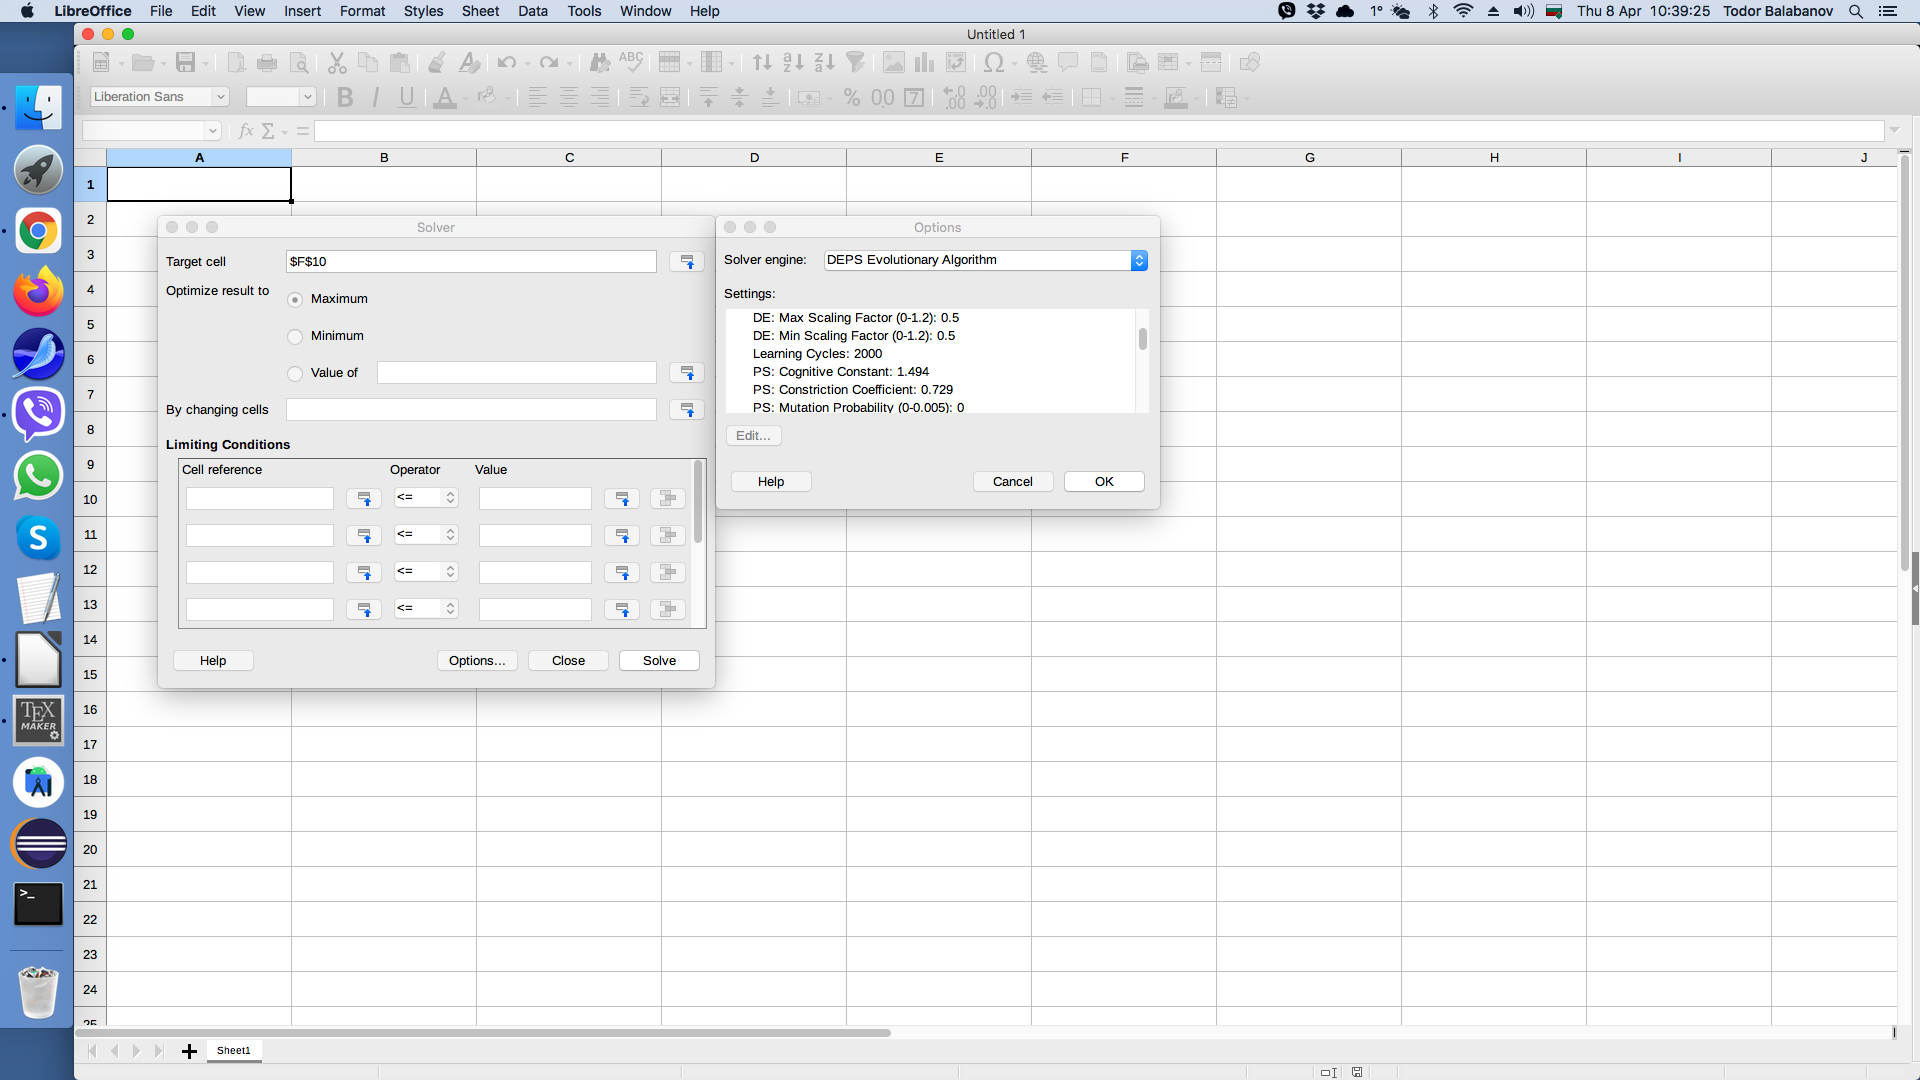
\includegraphics[width=1.0\linewidth]{fig001}
  \caption{Модул за оптимизация в LibreOffice Calc}
\label{fig001}
\end{figure}

За нелинейна оптимизация модулът прилага алгоритмите за еволюция на разликите и оптимизация с рояк от частици. Двата алгоритъма се прилагат в хибридна комбинация, като с предварително дефинирана вероятност е определено колко често ще бъде активиран всеки от тях. Модулът се настройва за клетка, чиято оптимална стойност ще бъде търсена (максимум, минимум или конкретно число). Също така, задава се и регионът от клетки, които подлежат на промяна в процеса по оптимизация. Като клетка в която ще се търси минимум при бързото протитипиране се избира общата средно-квадратична грешка допусната от изкуствената невронна мрежа. Регионът от клетки за оптимизация съдържа теглата използевани в изкуствената невронна мрежа. 

\begin{figure}[h]
  \centering
  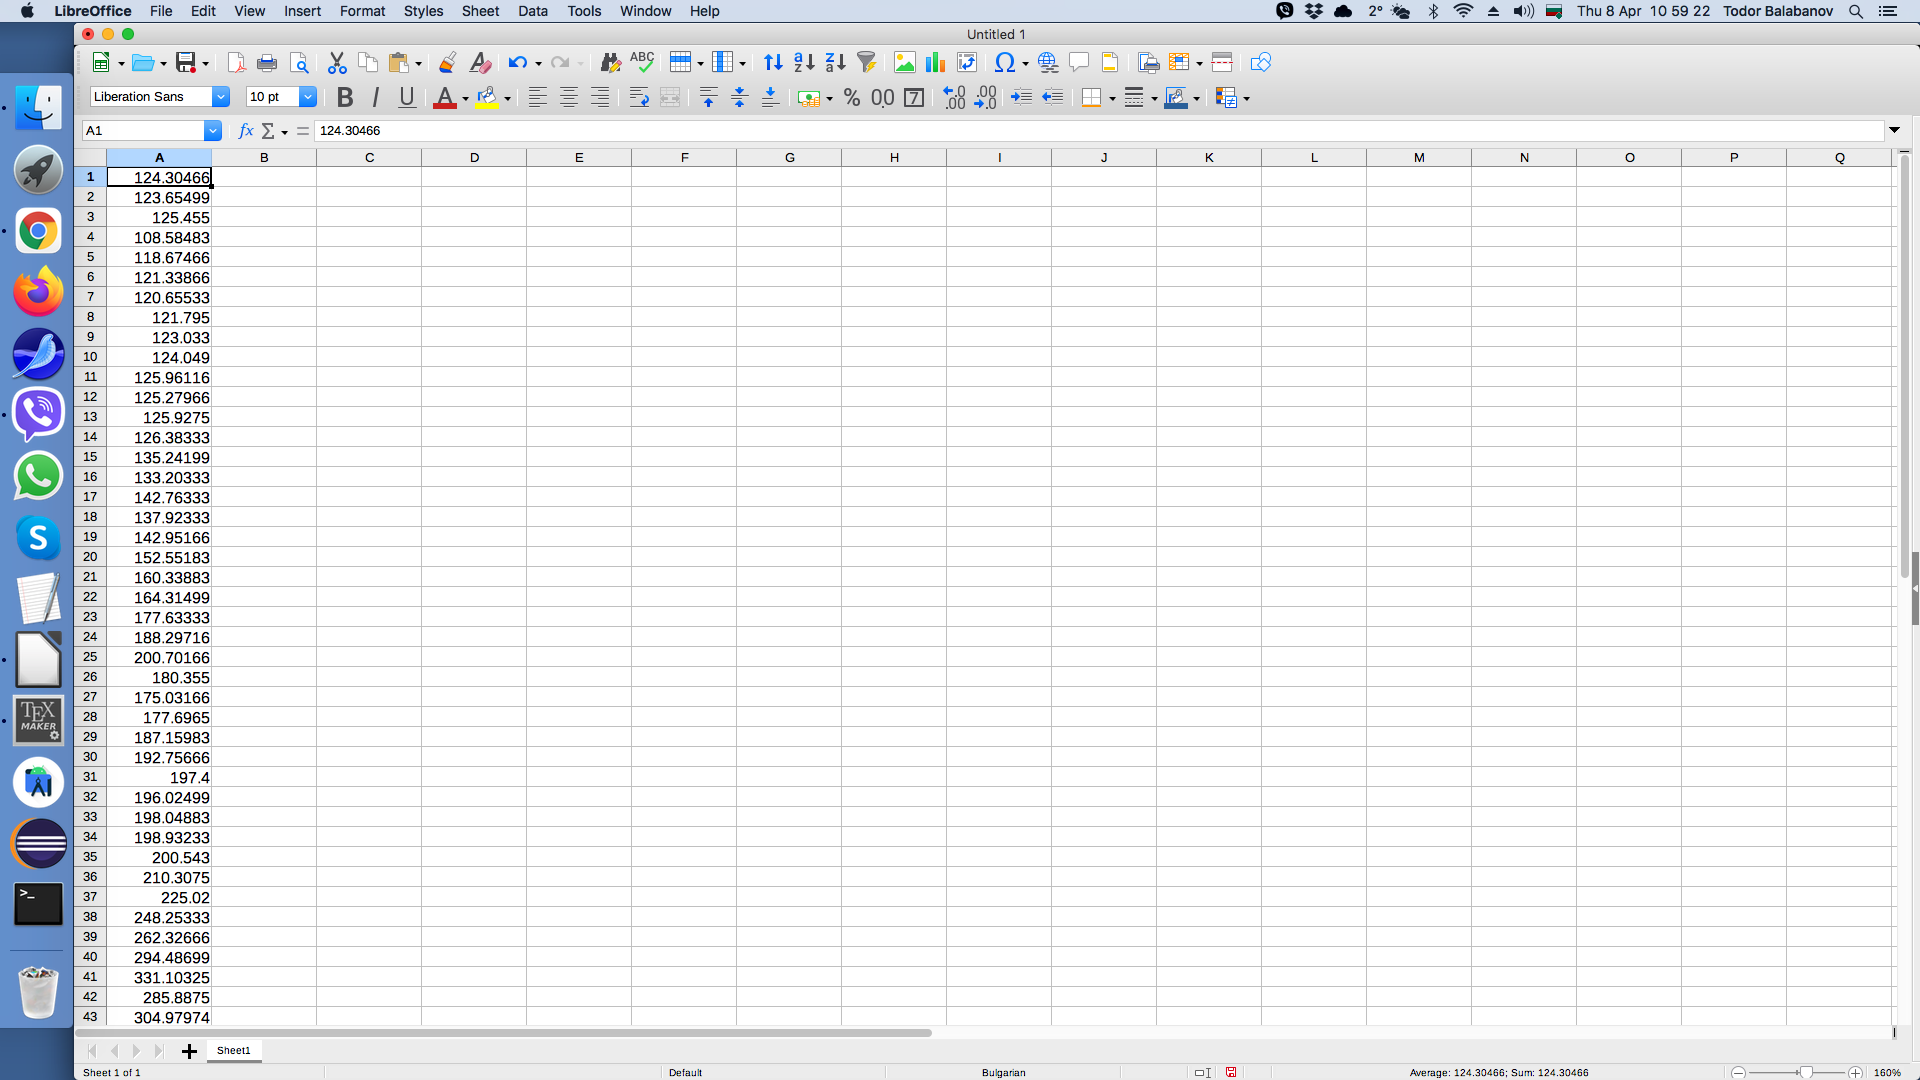
\includegraphics[width=1.0\linewidth]{fig002}
  \caption{Стойности на Bitcoin виртуалната валута}
\label{fig002}
\end{figure}

Като множество данни се използват стойностите на Bitcoin виртуалната валута (Фиг. \ref{fig002}), на дневна база, за няколко години назад. Моделът за прогнозиране се основава на нелинейна авторегресия. Това означава, че на входа на мрежата се подават мащабирани минали стойности от времевия ред, а на изхода на мрежата се очакват мащабирани прогнозни стойности. 

\begin{figure}[h]
  \centering
  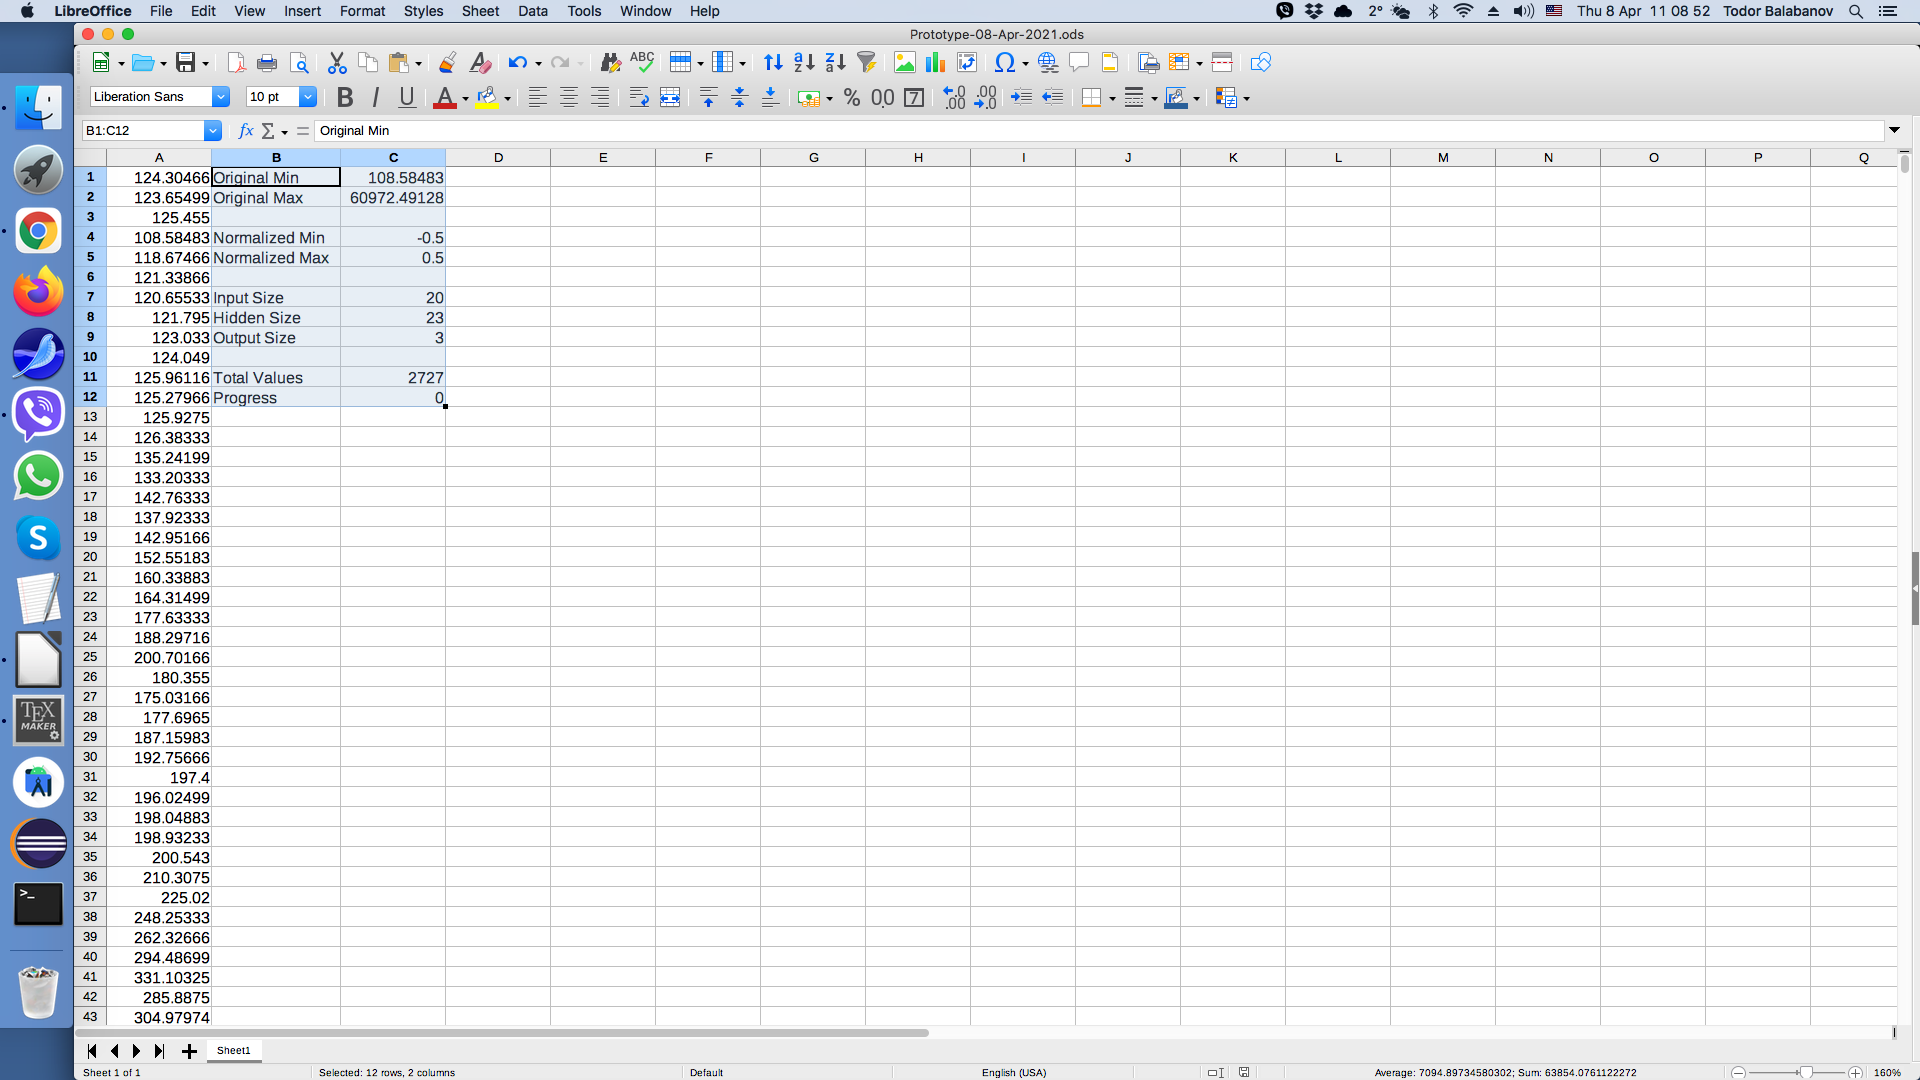
\includegraphics[width=1.0\linewidth]{fig003}
  \caption{Параметри на трислойната изкуствена невронна мрежа}
\label{fig003}
\end{figure}

След подбора на времеви ред следва избор на параметрите с които ще бъде напревен модела на трислойната изкуствена невронна мрежа (Фиг. \ref{fig003}). За целите на линейното мащабиране първо се намират най-малката и най-голямата стойност в оригиналния времеви ред, чрез формули в LibreOffice Calc: $=MIN(A:A)$ и $=MAX(A:A)$. Тъй като приложената прагова функция е хиперболичен тангенс, диапазона за мащабирания времеви ред е избран от -0.5 до +0.5. Умишлено се избягва мащабиране до асимптотичните стойности от -1.0 до +1.0, тъй като такова мащабиране много би увеличило стойностите на междинните пресмятания, а и не би дало възможност да се прогнозират по-малки или по-големи стойности от вече известните в оригиналния времеви ред. Топологията на мрежата се избира експериментално, като изходния слой има размер, според това колко стойности в бъдещето е желателно да се предсказват. Размера на входния слой се определя експериментално. За размера на скрития слой има различни емпирични правила, като най-популярното е скритият слой да бъде половината от сумата на размерите имащи входния и изходния слой. Съществуват адаптивни алгоритми, които чрез проби и грешки да определят топологията на мрежата, но в това бързо прототипиране тези алгоритми не се прилагат. 

Общият брой стойности в оригиналния времеви ред се определят с формула в  LibreOffice Calc: $=COUNT(A:A)$. Тъй като процеса по „разгръщането“ на модела е относително бавен, то се добавя клетка в която да се проследява напредъка от Python скрипта в „разгръщането“.


